\documentclass{article}

\usepackage[final]{corl_2026} % Camera-ready final version.
%\usepackage[preprint]{corl_2026} % Uncomment for a preprint version.
%\usepackage{corl_2026} % Use this for the submission version.

\usepackage[T1]{fontenc}
\usepackage[utf8]{inputenc}
\usepackage{microtype}
\usepackage{amsmath,amssymb}
\usepackage{amsthm}
\newtheorem{definition}{Definition}
\newtheorem{proposition}{Proposition}
\usepackage{booktabs}
\usepackage{graphicx}
\usepackage{float}
\usepackage{placeins}
\usepackage{multirow}
\usepackage{tikz}
\usetikzlibrary{positioning,arrows.meta,shapes.geometric}
\usepackage{pgfplots}
\usepgfplotslibrary{groupplots}
\pgfplotsset{compat=1.18}

% Shared macros for the paper export skeleton.
\newcommand{\task}[1]{\texttt{#1}}

\urlstyle{same}
\hypersetup{
  breaklinks=true
}

\title{When Does Memory Matter? A Diagnostic Framework for Partially Observable Manipulation}
\author{
Jiaming Xu\\
Harbin Institute of Technology\\
\texttt{2022110371@stu.hit.edu.cn}
\And
Danni Chang\\
Shanghai Jiao Tong University\\
\texttt{dchang1@sjtu.edu.cn}
}
\date{}

\begin{document}
\maketitle

% Export note:
% - Prose source: ../draft_v2.md
% - Bibliography source: ../references.bib
% - Numerical truth source: ../source_of_truth.md

\begin{abstract}
When a partially observable robot starts failing, the default reaction is often a monolithic one: upgrade the policy with ``more memory.'' We argue that this is an incomplete design question. The design problem is diagnostic: which task-relevant state was previously visible, which part of it must survive occlusion or sensing gaps, and what is the lowest-cost state-management intervention that restores control? We therefore frame manipulation under partial observability as a \emph{memory design triage} problem: first determine whether the failure is caused by previously seen state becoming hidden, then test whether a lightweight explicit cache is sufficient, and only then ask whether richer memory organization is warranted.

Using 9 MetaWorld tasks with controlled partial-observability protocols, we compare memory-free policies, flat-buffer memory policies, and structured memory policies under goal masking and joint goal-object masking. Under WeakPO, memory-free agents collapse to 0\% success on 7 of 9 tasks, whereas both memory variants recover to 51--100\% success with no significant difference between them. A zero-cost GoalBuffer also outperforms implicit recurrent memory under the same masking regime, supporting a \emph{cache-first diagnostic} for this task family. Under StrongPO, all tested goal-only variants fail, marking the boundary of \emph{goal-only memory}: once object state is hidden together with the goal, storing the goal alone cannot recover the missing state needed for control. Small cross-platform checks on FetchReach-v4 and FetchPush-v4 reproduce the same layered pattern. Overall, these results support a practical memory-management pipeline for single-goal manipulation under observation loss: diagnose the information bottleneck, try simple persistence first, and escalate to object-state access or belief estimation only when the lightweight explicit cache fails. We use the goal-dependency gradient $G(\tau)$ only as a lightweight screening signal for whether memory comparisons are worth running in this benchmark family, not as a general-purpose predictor of memory needs.
\end{abstract}

\keywords{robot manipulation, partial observability, memory}

\section{Introduction}
\label{sec:intro}

Real manipulation systems do not enjoy uninterrupted access to task state. In drawer opening, the robot may see the handle pose and desired opening direction on approach, then lose both as the gripper and cabinet frame block the wrist camera during contact. In object pushing, the puck location can be clear before contact and then disappear once the hand closes in, so the controller must continue from a partially remembered object state. In shelf placing, the target shelf slot may be visible during alignment but become hidden by the arm, shelf lip, or the carried object exactly when final placement requires precise correction. In these settings, the engineering problem is rarely ``should we add memory?'' in the abstract. The real question is how to \emph{triage} memory design: is the failure caused by hidden-but-previously-seen information, is a small cache enough to restore performance, or is the task actually demanding a richer state-management mechanism?

This distinction matters because partial observability, policy capacity, memory architecture, and recovery heuristics are often changed together. When they are confounded, a stronger result with a larger recurrent model does not tell us whether the bottleneck was missing information, missing persistence, or simply extra training capacity. Our thesis is that memory in these tasks should be treated not as a monolithic capacity upgrade, but as a targeted state-management decision about which previously observed variables must survive observation loss. We therefore study partial observability in manipulation as a \emph{memory-management pipeline}: first diagnose whether the task depends on retaining previously visible state, then test a lightweight explicit cache-first intervention, and only then ask whether richer memory structure or additional recovery logic is justified.

\paragraph{Research Questions.}
We therefore ask:
\begin{enumerate}
    \item[\textbf{Q1.}] When observations are masked but control and action primitives are fixed, does performance drop because task-relevant state must be preserved across time?
    \item[\textbf{Q2.}] If so, is a cache-first intervention---simple point-memory persistence of the last visible goal---already sufficient?
    \item[\textbf{Q3.}] Where is the boundary of that intervention: when do richer memory organization or recovery logic help, and when is the real problem that goal-only memory no longer contains the missing state?
\end{enumerate}

To answer these questions, we use a controlled setup on 9 MetaWorld \citep{Yu2020} tasks with two PO protocols---\emph{WeakPO} (goal masking) and \emph{StrongPO} (goal + object-position masking)---and three policy variants: \task{NoMemory} (no persistence), \task{TextBuffer} (flat goal cache), and \task{StructMemory} (key-value store). All three share the same finite-state controller, action primitives, and observation protocol; only the retained-state mechanism changes (Figure~\ref{fig:framework}). This lets us isolate a practical triage sequence: whether memory is needed at all, whether a simple cache is enough, and whether failures that survive caching actually point to a different memory boundary.

Our main contributions are:

\begin{enumerate}
    \item \textbf{We introduce a diagnostic framework for PO manipulation}: under a shared controller and masking protocol, we ask whether retained state is needed, whether a flat cache is sufficient, and whether any residual failure justifies richer memory or recovery.
    \item \textbf{We identify the boundary of goal-only memory}: contrasting WeakPO and StrongPO distinguishes cache-solvable hidden-goal failures from cases where hidden object or mechanism state pushes the task beyond goal persistence.
    \item \textbf{We derive a practical intervention rule}: begin with the lowest-cost explicit goal cache, move to object-state access or belief estimation when that fails, and reserve richer structure or recovery logic for the remaining cases.
\end{enumerate}

Taken together, these results define a practical memory-management pipeline for PO manipulation. First diagnose whether the hidden variable was previously observable and therefore recoverable by persistence. If yes, try the lowest-cost explicit cache intervention before investing in richer memory machinery. If that still fails, check whether the task has crossed the boundary of goal-only memory and now requires object-state access, object buffers, or belief estimation rather than better formatting of the cached goal. We summarize the task-side signal with a \emph{goal-dependency gradient}, but use $G(\tau)$ only as a lightweight screening heuristic for whether memory comparisons are worth running in this benchmark family, not as a universal proxy for memory requirements.

\input{figures/fig_framework}
\section{Related Work}
\label{sec:related-work}

\paragraph{POMDP and belief-space planning.}
POMDP methods provide the standard formalism for acting under hidden state \citep{Kaelbling1998, Spaan2012, Lauri2023}, and online planners such as POMCP \citep{Silver2010} demonstrate the value of maintaining beliefs over latent state. In manipulation, belief-space replanning can also be necessary for long-horizon tasks with uncertainty \citep{Garrett2020}. This literature establishes that hidden state should be reasoned about explicitly, but it usually targets full inference or planning over latent state rather than a systems-level triage question: before escalating to belief estimation, can a \emph{memory design diagnostic layer} first determine whether the failure is merely hidden previously visible state that only needs to be persisted?

\paragraph{Learned memory architectures.}
Another line of work equips policies with implicit learned memory through recurrent networks \citep{Hausknecht2015}, state-space models \citep{Gu2022}, transformers \citep{Vaswani2017, Brohan2023}, sequence modeling \citep{Chen2021}, world models \citep{Ha2018, Hafner2020}, image-based RL \citep{Yarats2021}, and meta-learning under partial observability \citep{Zintgraf2020}. These methods are often powerful because they combine representation learning, temporal abstraction, and memory in one end-to-end policy. However, that strength also makes diagnosis harder: when performance improves, it is often unclear whether the gain comes from genuinely retaining missing information, from larger model capacity, or from broader changes in training dynamics. What remains underspecified is the diagnostic layer that would justify invoking these heavy mechanisms in the first place, rather than first testing whether explicit low-cost persistence already removes the failure mode.

\paragraph{Explicit cache and goal memory.}
Work on explicit history modeling shows that structured access to past observations can improve manipulation \citep{Guhur2022}, and RoboMME suggests that different memory formats help on different task families \citep{Dai2026}. A related thread studies explicit goal caching or latent goal persistence \citep{Yarats2022, Lynch2020}, which is especially relevant when the missing variable was visible earlier and is compact enough to store directly. This line is closest to our setting because it points to a lightweight memory mechanism that is interpretable and controllable. Yet prior work typically evaluates such memory as one design option among many, rather than positioning it inside a diagnostic layer that asks whether a flat cache should be the first intervention and whether richer memory organization is warranted only after that cache fails.

\paragraph{Recovery policies.}
Recovery policies and retry mechanisms can improve robustness in sequential manipulation under noise and partial observability \citep{Vats2024, Vats2023}. They provide a different axis of adaptation: instead of preserving hidden state better, they alter control behavior after failure or uncertainty is detected. Such methods can be highly effective, but they also consume time, actions, and finite-horizon budget, so a stronger recovery policy is not automatically a lower-cost or cleaner fix than better state persistence. This creates another missing piece for a memory design diagnostic layer: before adding recovery logic, one should know whether the underlying failure is actually a persistence problem that a simple cache would solve more directly.

\paragraph{Gap.}
Taken together, prior work offers strong tools for hidden-state inference, learned memory, explicit caching, and recovery, but not a single \emph{memory design diagnostic layer} that orders them by necessity. The missing question is not simply ``which memory architecture scores highest?'' but ``what is the smallest intervention that plausibly addresses this failure mode?'' Our paper fills that gap by inserting an explicit diagnostic layer ahead of architecture escalation: first test whether hidden previously visible state is the relevant bottleneck, then test whether flat goal persistence already closes the gap, then ask whether richer organization or recovery adds anything beyond that cache, and finally mark the boundary where the missing state has moved beyond goal-only memory. This decision-oriented framing is the main distinction from prior memory or recovery comparisons.

\section{Method}
\label{sec:method}

We frame the method as a \emph{controlled diagnostic design} for partial observability, not as a search for the most powerful policy class. The key identification choice is therefore to hold the control policy class fixed while varying only the retained-state mechanism. All policy variants use the same finite-state-machine (FSM) controller, the same hand-written transition logic, the same action primitives, and the same observation interface; they differ only in how previously seen task-relevant information is retained after the goal becomes hidden. This fixed FSM is a deliberate controlled scaffold, not a methodological shortcut. If we changed controller capacity, exploration behavior, or action vocabularies together with memory, any success difference could always be attributed to increased controller capacity, leaving the memory question unanswered. By freezing those factors, we make retained state the only manipulated variable and can interpret the resulting memory gap as controlled evidence about \emph{what information must survive occlusion} rather than about which controller is more expressive \citep{Kaelbling1998}. Our claim is therefore intentionally narrower but cleaner: within a matched control backbone, does persistence alone repair the PO failure, and where does that repair stop working?

\subsection{Controlled Diagnostic Family}

\begin{itemize}
\item \task{NoMemory} uses the shared controller without retaining goal information after the initial observation.
\item \task{TextBuffer} uses the same controller and primitives, but retains the goal position in a lightweight flat buffer.
\item \task{StructMemory} uses the same controller and primitives, but retains the same core content in a key-value format with typed fields and event records (FSM state, retry count, rollback flag).
\end{itemize}

All three variants execute the same five-stage grasp sequence (approach $\to$ descend $\to$ grasp $\to$ lift/move $\to$ release) through the same fixed action primitives. This shared controller should not be read as assuming that real robots ought to use FSMs universally. It is the minimal matched scaffold that makes the diagnostic identifiable: if a flat cache and a structured store produce different outcomes under the same primitives, the difference is attributable to retained state; if they do not, then richer memory formatting is not the active ingredient in this benchmark family. The variant-to-question mapping is:
\begin{center}
\footnotesize
\setlength{\tabcolsep}{5pt}
\begin{tabular}{lll}
\hline
Variant & Question & Diagnostic target \\
\hline
\task{NoMemory} & Q1 & memory necessity \\
\task{TextBuffer} & Q2 & point-memory sufficiency \\
\task{StructMemory} & Q3 & beyond-persistence benefit \\
\hline
\end{tabular}
\end{center}
Equivalently, \task{NoMemory} asks whether retained state is needed at all, \task{TextBuffer} asks whether simple persistence is sufficient, and \task{StructMemory} asks whether richer organization improves over simple persistence. Because the retained-state mechanism is the only changing factor, contrasts among these variants directly implement the three diagnostic questions rather than merely comparing unrelated policies. Our retry ablations later probe the same Q3 axis from the control side by asking whether additional recovery logic helps, or instead consumes finite-horizon budget.

\subsection{Partial-Observability Protocol}

The PO wrapper masks task-relevant observations after the initial step and exposes the goal for one step every \texttt{flash\_every} steps (default: 20), controlled by \texttt{flash\_len} (default: 1). We define two diagnostic protocols:
\begin{itemize}
\item \textbf{Weak PO}: masks goal position only, so any success difference isolates the need to retain previously observed goal information.
\item \textbf{Strong PO}: masks both goal and object positions, so the diagnosis tests whether performance also depends on retained manipulated-object state rather than goal information alone.
\end{itemize}
Figure~\ref{fig:flash_every} in the appendix varies \texttt{flash\_every} across $\{1, 5, 10, 20, 50\}$ to control PO severity directly.

\subsection{Controlled Diagnostic Logic}

We formalize three progressively stronger diagnostic layers as a strict hierarchy:

\begin{definition}[Memory Necessity]
The \emph{memory gap} is
\[
\Delta_{\text{mem}}(\tau) = \max_{\pi \in \{\text{TB}, \text{SM}\}} S(\pi, \tau, \text{PO}) - S(\text{NM}, \tau, \text{PO}).
\]
Memory is \emph{necessary} iff $\Delta_{\text{mem}}(\tau) > 0$ with $p < 0.05$.
\end{definition}

Because \task{NoMemory}, \task{TextBuffer}, and \task{StructMemory} share the same FSM controller and fixed action primitives, while differing only in retained-state mechanism, $\Delta_{\text{mem}}(\tau)$ supports a controlled-ablation interpretation inside this benchmark family: it measures the success gain associated with adding retention to an otherwise unchanged controller.

\begin{definition}[Structure Differentiation]
The \emph{structure gap} is
\[
\Delta_{\text{struct}}(\tau) = |S(\text{TB}, \tau, \text{PO}) - S(\text{SM}, \tau, \text{PO})|.
\]
Structure \emph{differentiates} iff $\Delta_{\text{struct}}(\tau) > 0$ with significance; otherwise, the task requires only \emph{point memory}.
\end{definition}

\begin{definition}[Goal-Dependency Gradient]
\[
G(\tau) = S(\text{NM}, \tau, \text{FO}) - S(\text{NM}, \tau, \text{PO}).
\]
We use $G(\tau)$ as a \emph{diagnostic screening signal}: in our 9-task suite, $G(\tau) > 0.5$ marks \emph{high-dependency} tasks and $G(\tau) < 0.1$ marks \emph{low-dependency} tasks.
\end{definition}

\begin{proposition}[Diagnostic Layers]
Layer 1 tests whether hidden information matters ($\Delta_{\text{mem}}(\tau) > 0$). Layer 2 tests whether simple persistence is sufficient ($S(\text{TB}, \tau, \text{PO}) \approx S(\text{TB}, \tau, \text{FO})$). Layer 3 tests whether richer organization adds value ($\Delta_{\text{struct}}(\tau) > 0$). Each diagnostic layer subsumes the previous one.
\end{proposition}

Together, these diagnostic layers define a lightweight controlled workflow. We first estimate or measure the \task{NoMemory} FO-to-PO gap $G(\tau)$ as a screening signal for whether a memory comparison is worth running at all. We then interpret $\Delta_{\text{mem}}(\tau)$ as the gain associated with adding retained state to the shared controller, and $\Delta_{\text{struct}}(\tau)$ as the incremental gain associated with organizing that retained state more richly. The diagnostic outcome therefore localizes the dominant bottleneck to one of three places: observability itself, memory persistence, or memory structure.

\subsection{Goal-Relative Extension}

For contact-rich tasks, we introduce a \emph{Goal-Relative} extension: every goal-oriented stage reads \texttt{obs.goal\_pos} at every step. When the goal is masked (zero), the stage returns zero action. This prevents cached-goal leakage; otherwise, the shared FSM controller could bypass the PO mask via previously cached goal information.

\section{Experimental Setup}
\label{sec:experimental-setup}

We evaluate 9 MetaWorld \citep{Yu2020} tasks with vector observations to separate information loss, memory retention, and recovery cost under a shared PO protocol.

\subsection{Tasks}

\textbf{Core tasks} (3 tasks, V1 FSM): \task{reach-v3}, \task{push-v3}, \task{pick-place-v3}. \textbf{Contact-rich tasks} (6 tasks, V2 Goal-Relative FSM): \task{door-open-v3}, \task{drawer-open-v3}, and \task{faucet-open-v3}. The remaining contact-rich tasks are \task{button-press-topdown-v3}, \task{sweep-v3}, and \task{shelf-place-v3}. We omit \task{basketball-v3} because it largely duplicates the staged transport structure of \task{pick-place-v3} while adding little variation in memory demand.

\subsection{Evaluation Protocol}

Rule-based experiments use 5 seeds; learned policies and cross-platform checks use 3; each seed runs 60 episodes with a 200-step cap. Success rate is the primary metric, standard deviation is reported throughout, and permutation tests assess significance \citep{Good2005}.

\subsection{Learned Policy Baselines}

To test whether learned policies show the same PO vulnerability, we train SAC \citep{Haarnoja2018} agents with MLP and LSTM \citep{Hochreiter1997} backbones for 500K--2M steps under FO or PO, then evaluate them under FO, WeakPO, and StrongPO. We additionally test a zero-cost GoalBuffer that caches the last visible goal and restores masked goal dimensions at evaluation time. For a small cross-platform check, Table~\ref{tab:cross_platform} in the appendix repeats the rule-based protocol on FetchReach-v4 and FetchPush-v4 \citep{DeLazcano2023}.

\section{Results}
\label{sec:results}

We organize the results as the same layered diagnostic procedure introduced above. Layer 1 tests whether WeakPO creates an information bottleneck; Layers 2--3 test whether persistence is sufficient and whether structure changes the diagnosis; the final layer tests whether recovery is worth its finite-horizon cost. StrongPO then marks where the bottleneck shifts beyond goal-only memory.

\subsection{Memory Is Necessary (Layer 1)}

Diagnostic Layer 1 asks whether removing memory exposes a meaningful information bottleneck under WeakPO.

Table~\ref{tab:main_results} shows that \task{NoMemory} collapses under WeakPO in 7/9 tasks ($p < 0.01$). The main exception is Button-Press, whose downward motion is strongly constrained by geometry and appears nearly goal-independent ($G=-0.01$). The resulting memory gap $\Delta_{\text{mem}}$ spans 0.0--1.0, suggesting that PO usually introduces a substantial information bottleneck in this suite.

\begin{table}[t]
\centering
\caption{Success rates (\%) on 9 MetaWorld tasks under Full-Observable (FO) and WeakPO conditions (\texttt{flash\_every}$=$20). Entries are mean $\pm$ std over 5 seeds $\times$ 60 episodes. \textbf{NM} = NoMemory, \textbf{TB} = TextBuffer, \textbf{SM} = StructMemory. $\dagger$ marks V1 FSM tasks; all others use V2 Goal-Relative FSM. $^{**}$ marks $p < 0.01$ for NM FO vs.\ WeakPO.}
\label{tab:main_results}
\resizebox{\textwidth}{!}{%
\begin{tabular}{l ccc c ccc c c}
\toprule
& \multicolumn{3}{c}{FO} & & \multicolumn{3}{c}{WeakPO} & & \\
\cmidrule(lr){2-4} \cmidrule(lr){6-8}
Task & NM & TB & SM & & NM & TB & SM & & NM $\Delta$(WeakPO$-$FO) \\
\midrule
\multicolumn{10}{l}{\textit{Core Tasks (V1 FSM)$^\dagger$}} \\
Reach$^{**}$        & 82.3$\pm$9.5 & 82.3$\pm$9.5 & 82.3$\pm$9.5 & & 0.0$\pm$0.0 & 64.7$\pm$7.8 & 64.7$\pm$7.8 & & $-$82.3 \\
Push$^{**}$         & 64.3$\pm$29.7 & 66.0$\pm$28.5 & 64.3$\pm$29.7 & & 0.0$\pm$0.0 & 65.7$\pm$26.7 & 64.3$\pm$28.0 & & $-$64.3 \\
Pick-Place$^{**}$   & 74.0$\pm$7.1 & 74.0$\pm$7.1 & 74.0$\pm$7.1 & & 0.0$\pm$0.0 & 74.7$\pm$5.5 & 74.7$\pm$5.5 & & $-$74.0 \\
\midrule
\multicolumn{10}{l}{\textit{Extended Tasks (V2 Goal-Relative FSM)}} \\
Door-Open$^{**}$    & 90.3$\pm$5.7 & 91.0$\pm$5.1 & 90.3$\pm$5.7 & & 0.0$\pm$0.0 & 90.7$\pm$5.6 & 90.7$\pm$5.2 & & $-$90.3 \\
Drawer-Open$^{**}$  & 100.0$\pm$0.0 & 100.0$\pm$0.0 & 100.0$\pm$0.0 & & 0.0$\pm$0.0 & 100.0$\pm$0.0 & 100.0$\pm$0.0 & & $-$100.0 \\
Faucet-Open$^{**}$  & 56.3$\pm$5.6 & 54.0$\pm$3.8 & 56.3$\pm$5.6 & & 2.3$\pm$2.2 & 54.0$\pm$3.8 & 56.0$\pm$4.9 & & $-$54.0 \\
Button-Press        & 60.3$\pm$13.2 & 59.7$\pm$15.2 & 60.3$\pm$13.2 & & 61.3$\pm$13.9 & 60.7$\pm$13.3 & 58.7$\pm$15.2 & & $+$1.0 \\
Sweep$^{**}$        & 52.0$\pm$3.0 & 52.0$\pm$3.2 & 52.0$\pm$3.0 & & 0.0$\pm$0.0 & 51.0$\pm$3.2 & 51.7$\pm$2.4 & & $-$52.0 \\
Shelf-Place$^{**}$  & 89.0$\pm$6.3 & 84.7$\pm$5.2 & 89.0$\pm$6.3 & & 0.0$\pm$0.0 & 84.7$\pm$5.1 & 89.0$\pm$6.3 & & $-$89.0 \\
\bottomrule
\end{tabular}%
}
\end{table}


\subsection{Simple Persistence Is Sufficient for the Current Single-Goal Task Family (Layers 2--3)}

Diagnostic Layers 2--3 ask whether explicit persistence is enough once Layer 1 has established a bottleneck, and whether additional structure changes that diagnosis.

Both \task{TextBuffer} and \task{StructMemory} restore WeakPO performance to 51--100\% (Table~\ref{tab:main_results}), with $\Delta_{\text{struct}}<0.05$ and no significant difference across all 9 tasks. This suggests that, in the current single-goal suite, the decisive factor is persistence rather than richer organization of that memory. The same pattern holds in the sequential multi-goal setting (Table~\ref{tab:multi_goal} in the appendix), so the current suite appears to require only \emph{point memory}. Under StrongPO, however, all three goal-only variants collapse to 0\% across the 9 tasks (Appendix A.7), marking the boundary of the current goal-only intervention: once object position is also hidden, goal persistence alone is insufficient, and the next diagnostic layer should consider object-state buffers or belief estimation.

\input{figures/fig_goal_dependency}

\paragraph{Door-Open as a boundary case.}
Door-Open-v3 provides the strongest example of where Layer 1 and Layers 2--3 separate cleanly. In Table~\ref{tab:main_results}, \task{NoMemory} drops from 90.3\% under FO to 0.0\% under WeakPO, while both memory variants stay near 91\%, so the task is highly sensitive to losing the goal but comparatively insensitive to how that goal is stored. Figure~\ref{fig:flash_every} in the appendix sharpens this point: \task{NoMemory} already collapses at \texttt{flash\_every}$=5$, whereas \task{TextBuffer} and \task{StructMemory} overlap throughout. The same task also marks the StrongPO boundary, where all three goal-only variants collapse to 0\% once object state is hidden.

\subsection{Implicit Recurrent Memory vs.\ Explicit Persistence}
\label{sec:lstm_vs_goalbuffer}

This diagnostic layer asks whether implicit recurrent memory can substitute for explicit persistence once the need for memory has been established.

Table 2 and Figures 3--4 in Appendix A.1 compare learned and explicit memory. FO-trained SAC-MLP reaches 78.9--100\% under FO but collapses to 0--1.1\% under WeakPO. SAC-LSTM provides partial robustness on Reach-v3 (42.2\%) and highly variable behavior on Faucet-Open-v3 ($\sigma=41.4\%$), while a zero-cost GoalBuffer recovers WeakPO to 82.2--100\% on five tasks without retraining. In this diagnostic reading, implicit recurrent memory does not appear to reliably replace explicit persistence for the present observation-masking intervention, although the comparison remains limited to these tasks and training settings.

\subsection{Recovery and Finite-Horizon Cost}
\label{sec:recovery_cost}

This recovery layer asks whether adding recovery behavior is worth its finite-horizon cost.

Retry provides no measurable benefit on single-phase tasks and reduces performance on Pick-Place: under a 200-step budget, rollback consumes steps needed for the place phase ($-54.4$pp; Table~\ref{tab:retry} in the appendix). For the current horizon and task structure, the evidence suggests that recovery is usually not worth its cost unless the expected gain from correcting an earlier failure exceeds the steps spent on rollback. Figure~\ref{fig:flash_every} in the appendix further shows that the WeakPO bottleneck scales smoothly with flash sparsity.

\paragraph{Cross-platform sanity-check.}
Table~\ref{tab:cross_platform} in the appendix repeats the rule-based protocol on FetchReach-v4 and FetchPush-v4. Despite the different robot platform and task suite, the same layered pattern reappears: \task{NoMemory} degrades under WeakPO, while both memory variants recover to FO-level performance. This small sanity-check is consistent with the MetaWorld diagnosis that the main bottleneck is hidden state, and that carrying the missing goal information forward matters more here than the particular organization imposed on that memory.

\FloatBarrier

\section{Discussion}
\label{sec:discussion}

\paragraph{When does memory matter?}
Memory matters when task-relevant state is hidden and must be carried across time to select the right action. In this task family, that state is usually the hidden goal under WeakPO: \task{NoMemory} fails on 7/9 tasks, while either memory-enabled variant recovers. This indicates that the dominant failure is an \emph{information-management} problem before it is a model-capacity problem.

\paragraph{Why does simple persistence suffice here?}
The current tasks primarily require point memory: preserving the hidden goal matters more than how that value is packaged. This is why the paper should be read as a diagnostic result, not as a broad ranking of memory architectures. We expect $\Delta_{\text{struct}}>0$ mainly outside this single-goal regime, for example in tasks involving object identity, relational state, or ordered subgoals.

\paragraph{Failure mode and practical implication.}
WeakPO exposes goal-seeking failure, which is largely resolved by goal memory. StrongPO exposes object-localization failure, where goal-only memory is insufficient and the next intervention should be object-state estimation, object buffers, or belief estimation. Thus, for this benchmark family, the practical order is \emph{cache first, learned recurrent memory second, structured memory third}, with recovery treated separately because retries and rollback consume finite-horizon budget.

\section{Limitations}
\label{sec:limitations}

Our study has three main limitations. First, the tasks are drawn from MetaWorld with low-dimensional vector observations; high-dimensional visual observations may reveal different memory requirements. Second, the PO protocols are synthetic and periodic, whereas real-world PO may be stochastic and task-dependent. Third, the current tasks primarily require point memory, so tasks involving multiple objects, object identity, relational state, mechanism uncertainty, or ordered subgoals may produce a nonzero structure gap. We therefore do not claim a universal ranking of memory architectures or direct sim-to-real transfer of the tested controllers. The purpose of the controlled benchmark is narrower: to isolate whether PO failure is caused by loss of previously observed state, insufficient persistence, or hidden object state that requires estimation.

Similarly, StrongPO should not be read as showing that memory is useless when object state is hidden. It is a boundary test: goal-only memory becomes insufficient, and the relevant next-step interventions are object-state estimation, object buffers, or belief estimation. The experiments bound where simple goal caching succeeds and where a different state-management layer is required.

\section{Conclusion}
\label{sec:conclusion}

We presented a layered diagnostic of partial observability in manipulation. Memory matters when task-relevant state is hidden and must be preserved across time, but the correct intervention depends on which state is missing. In this task family, that usually means hidden goal information under WeakPO; once that information is retained, the decisive factor is persistence rather than memory organization. The main thesis is therefore not that one buffer universally beats another, but that under goal-centric PO, cache-first mechanisms often solve the active bottleneck.

StrongPO sharpens the boundary: once hidden state includes object or mechanism state, goal caching is insufficient and the problem shifts toward object-state estimation, object buffers, or belief estimation. Future work should test whether relational, multi-object, or long-horizon sequential tasks produce the nonzero $\Delta_{\text{struct}}$ that is absent here, and whether the proposed diagnostic continues to identify when the bottleneck is persistence, estimation, or richer memory organization.


\clearpage
\acknowledgments{We thank the reviewers for their constructive feedback. We also thank our colleagues and advisors for valuable discussions and support during the development of this work.}

\bibliography{../references}

\clearpage
\appendix
\section{Appendix}
\label{sec:appendix}

\FloatBarrier

\subsection{Learned-Policy Comparison and GoalBuffer Recovery}

This subsection receives the learned-policy comparison block referenced from the main text. Table~\ref{tab:sac_baselines} together with Figures~\ref{fig:three_way}--\ref{fig:goalbuffer} compare learned and explicit memory, and we keep this evidence block here so that Table~\ref{tab:sac_baselines} stays in the appendix rather than drifting toward the conclusion.

\begin{table}[t]
\centering
\caption{Learned-policy comparison under FO, WeakPO, and StrongPO. SAC-MLP is trained under FO for 2M steps; SAC-LSTM under WeakPO for 2M steps. Entries are success rates (\%), reported as mean $\pm$ std over 3 seeds $\times$ 60 episodes unless marked $^\dagger$ (single seed). WeakPO masks goal position; StrongPO also masks object position (\texttt{flash\_every}$=$5, \texttt{flash\_len}$=$1).}
\label{tab:sac_baselines}
\begin{tabular}{l ccc}
\toprule
Task & Condition & SAC-MLP (FO-train) & SAC-LSTM (PO-train) \\
\midrule
\multirow{3}{*}{Reach-v3}
 & FO        & 78.9$\pm$6.0  & 47.8$\pm$9.0  \\
 & WeakPO    &  0.0$\pm$0.0  & 42.2$\pm$5.9  \\
 & StrongPO  &  0.0$\pm$0.0  & 29.4$\pm$6.5  \\
\midrule
\multirow{3}{*}{Faucet-Open-v3}
 & FO        & 100.0$\pm$0.0 & 74.4$\pm$35.6 \\
 & WeakPO    &   1.1$\pm$1.9 & 72.8$\pm$41.4 \\
 & StrongPO  &   5.0$\pm$8.7 &   1.1$\pm$1.9 \\
\midrule
\multirow{3}{*}{Door-Open-v3$^\dagger$}
 & FO        & 100.0 (n=1)   & ---            \\
 & WeakPO    &   0.0 (n=1)   & ---            \\
 & StrongPO  &   0.0 (n=1)   & ---            \\
\midrule
\multirow{3}{*}{Drawer-Open-v3$^\dagger$}
 & FO        & 100.0 (n=1)   & ---            \\
 & WeakPO    &  20.0 (n=1)   & ---            \\
 & StrongPO  &   0.0 (n=1)   & ---            \\
\bottomrule
\end{tabular}
\begin{flushleft}
\footnotesize SAC-MLP collapses under PO on all four tasks. SAC-LSTM shows high variance on Faucet-Open-v3 and trades FO performance for partial PO robustness on Reach-v3. GoalBuffer recovers WeakPO to 82--100\% without retraining (Table~\ref{tab:goal_buffer}). $^\dagger$ denotes single-seed SAC-MLP results; Pick-Place/Push/Button-Press are excluded because FO learning does not become reliable within 2M steps.
\end{flushleft}
\end{table}

\begin{figure}[t]
\centering
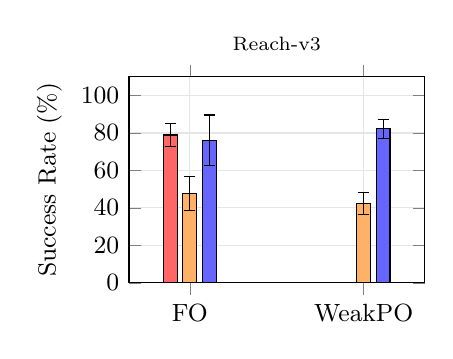
\begin{tikzpicture}
\begin{axis}[
    ybar,
    width=0.44\textwidth,
    height=4.2cm,
    bar width=5pt,
    ymin=0, ymax=110,
    ytick={0,20,40,60,80,100},
    symbolic x coords={FO, WeakPO},
    xtick=data,
    enlarge x limits=0.35,
    grid=major,
    grid style={gray!20},
    ylabel={Success Rate (\%)},
    error bars/y dir=both,
    error bars/y explicit,
    tick label style={font=\small},
    label style={font=\small},
    title={\scriptsize Reach-v3},
]
\addplot[fill=red!60] coordinates {(FO,78.9) +- (0,6.0) (WeakPO,0.0) +- (0,0.0)};
\addplot[fill=orange!60] coordinates {(FO,47.8) +- (0,9.0) (WeakPO,42.2) +- (0,5.9)};
\addplot[fill=blue!60] coordinates {(FO,76.1) +- (0,13.5) (WeakPO,82.2) +- (0,5.0)};
\end{axis}
\end{tikzpicture}
\hfill
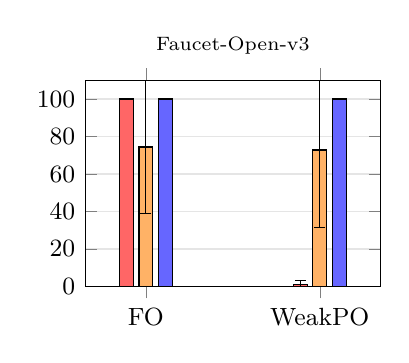
\begin{tikzpicture}
\begin{axis}[
    ybar,
    width=0.44\textwidth,
    height=4.2cm,
    bar width=5pt,
    ymin=0, ymax=110,
    ytick={0,20,40,60,80,100},
    symbolic x coords={FO, WeakPO},
    xtick=data,
    enlarge x limits=0.35,
    grid=major,
    grid style={gray!20},
    error bars/y dir=both,
    error bars/y explicit,
    tick label style={font=\small},
    title={\scriptsize Faucet-Open-v3},
]
\addplot[fill=red!60] coordinates {(FO,100.0) +- (0,0.0) (WeakPO,1.1) +- (0,1.9)};
\addplot[fill=orange!60] coordinates {(FO,74.4) +- (0,35.6) (WeakPO,72.8) +- (0,41.4)};
\addplot[fill=blue!60] coordinates {(FO,100.0) +- (0,0.0) (WeakPO,100.0) +- (0,0.0)};
\end{axis}
\end{tikzpicture}
\par\vspace{1mm}
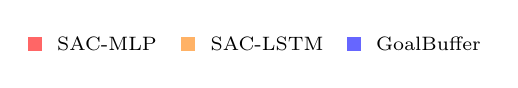
\begin{tikzpicture}[baseline]
\fill[red!60] (0,0) rectangle (0.18,0.18);
\node[anchor=west, font=\scriptsize] at (0.25,0.09) {SAC-MLP};

\fill[orange!60] (1.95,0) rectangle (2.13,0.18);
\node[anchor=west, font=\scriptsize] at (2.20,0.09) {SAC-LSTM};

\fill[blue!60] (4.05,0) rectangle (4.23,0.18);
\node[anchor=west, font=\scriptsize] at (4.30,0.09) {GoalBuffer};
\end{tikzpicture}
\caption{Three-way comparison on Reach-v3 and Faucet-Open-v3. Bars show mean over 3 seeds $\times$ 60 episodes; error bars denote std. SAC-LSTM is high-variance on Faucet-Open-v3 ($\sigma=41.4\%$), while GoalBuffer recovers WeakPO to 82.2--100\% on both tasks.}
\label{fig:three_way}
\end{figure}

\input{figures/fig_goalbuffer}

\FloatBarrier

\input{figures/fig_flash_every}

\subsection{Task Details}

All 9 tasks use the MuJoCo \citep{Todorov2012} simulator via MetaWorld V3 \citep{Yu2020} with 200-step episodes. Observation dimensions range from 10 (Reach-v3) to 23 (Pick-Place-v3); action dimension is 4 for all tasks. Rule-based experiments use fixed seeds $\{0,1,2,3,4\}$; learned policies and Gymnasium-Robotics use $\{0,1,2\}$.

\subsection{PO Wrapper Implementation}

The PO wrapper operates on the observation vector: on non-flash steps, it zeros out the goal position (WeakPO) or both goal and object positions (StrongPO). The flash schedule is deterministic: the goal is revealed for \texttt{flash\_len} steps every \texttt{flash\_every} steps, starting from step 0.

\subsection{SAC Hyperparameters}

\begin{itemize}
\item Learning rate: 3e-4 (actor and critic)
\item Discount factor $\gamma$: 0.99
\item Soft update coefficient $\tau$: 0.005
\item Replay buffer size: 1,000,000
\item Batch size: 256
\item Training starts at step 10,000
\item MLP: 2 hidden layers of 256 units with ReLU
\item LSTM: 128 hidden units, unroll length 20
\end{itemize}

\subsection{GoalBuffer Implementation}

See \S\ref{sec:experimental-setup} for the GoalBuffer definition. Under StrongPO, the object position remains masked (not cached), which is why GoalBuffer only partially recovers StrongPO performance.

\subsection{Push-v3 Variance Analysis}

Push-v3 shows high variance across seeds under FO (mean 64.3\%, std 29.7\%). This is because the task is near the boundary of open-loop solvability: some seeds place the arm close enough to the goal that the push succeeds regardless of observation, while others require precise goal-relative positioning. This variance is not an artifact of our framework but reflects the task's moderate goal-dependency ($G = 0.64$).

\subsection{StrongPO Full Results}

Under StrongPO, all 9 tasks $\times$ 3 rule-based policy variants yield 0.0$\pm$0.0\% success rate (5 seeds $\times$ 60 episodes). The complete results are visualized in Figure~\ref{fig:goal_dependency}.

\subsection{Door-Open-v3 Learned-Policy Single-Seed Limitation}

This subsection refers to the SAC-MLP learned-policy result in Table~\ref{tab:sac_baselines}. Door-Open-v3 seed 0 achieves 100\% under FO but 0\% under both WeakPO and StrongPO. Seeds 1--2 were not completed within the training budget. We present seed 0 as a single-seed limitation case for the learned SAC-MLP baseline: under this trained policy and masking protocol, sustained contact with a partially observed mechanism is not recovered without an explicit goal buffer or additional state estimation.

Drawer-Open-v3 (seed 0, single seed) achieves FO 100.0 / WeakPO 20.0 / StrongPO 0.0. The non-zero WeakPO result likely reflects that the initial drawer configuration provides partial goal information through object state before the goal is masked.

\subsection{Full Flash-Every Ablation Results}

Figure~\ref{fig:flash_every} above visualizes the flash-every ablation for Reach-v3 and Door-Open-v3. Table~\ref{tab:flash_every} provides the full numerical results for these two tasks across all flash frequencies. Table~\ref{tab:flash_every_full} reports the remaining tasks. This ablation was run as an independent 5-seed batch from Table~\ref{tab:main_results}; therefore the \texttt{flash\_every}$=20$ rows can differ slightly from the main-table PO numbers. The pattern is consistent: NoMemory degrades monotonically with increasing flash interval, while TextBuffer and StructMemory remain near-FO performance across all flash frequencies.

\begin{table}[t]
\centering
\caption{Success rates (\%) under varying goal flash frequency (\texttt{flash\_every}). Mean $\pm$ std over 5 seeds $\times$ 60 episodes. At \texttt{flash\_every}$=k$, the goal is visible for 1 step every $k$ steps; $k$=1 means goal visible every step (FO equivalent).}
\label{tab:flash_every}
\begin{tabular}{l ccc}
\toprule
flash\_every & NoMemory & TextBuffer & StructMemory \\
\midrule
\multicolumn{4}{l}{\textit{Reach-v3}} \\
1  & 82.3$\pm$9.5 & 82.3$\pm$9.5 & 82.3$\pm$9.5 \\
5  & 38.7$\pm$9.5 & 75.0$\pm$6.4 & 75.0$\pm$6.4 \\
10 & 4.0$\pm$8.0 & 73.7$\pm$9.5 & 73.7$\pm$9.5 \\
20 & 0.0$\pm$0.0 & 69.7$\pm$6.1 & 69.7$\pm$6.1 \\
50 & 0.0$\pm$0.0 & 60.0$\pm$7.1 & 60.0$\pm$7.1 \\
\midrule
\multicolumn{4}{l}{\textit{Door-Open-v3}} \\
1  & 90.3$\pm$5.7 & 91.0$\pm$5.1 & 90.3$\pm$5.7 \\
5  & 0.0$\pm$0.0 & 91.0$\pm$5.1 & 90.7$\pm$5.2 \\
10 & 0.0$\pm$0.0 & 90.7$\pm$5.6 & 91.0$\pm$4.8 \\
20 & 0.0$\pm$0.0 & 90.7$\pm$5.6 & 90.7$\pm$5.2 \\
50 & 0.0$\pm$0.0 & 91.0$\pm$5.1 & 91.0$\pm$4.8 \\
\bottomrule
\end{tabular}
\end{table}

\begin{table}[t]
\centering
\caption{Success rates (\%) under WeakPO with varying \texttt{flash\_every} for Push-v3, Pick-Place-v3, and Sweep-v3. Mean $\pm$ std over 5 seeds $\times$ 60 episodes. Caveat: this table comes from the independent flash-frequency ablation batch described above, so the \texttt{flash\_every}$=20$ rows can differ slightly from Table~\ref{tab:main_results}; the FO-equivalent \texttt{flash\_every}$=1$ case is omitted because it is already reported in Table~\ref{tab:flash_every}.}
\label{tab:flash_every_full}
\begin{tabular}{l cccc}
\toprule
Task & flash\_every & NoMemory & TextBuffer & StructMemory \\
\midrule
\multirow{4}{*}{Push-v3}
 & 5  & 41.7$\pm$39.1 & 66.3$\pm$23.9 & 64.3$\pm$24.7 \\
 & 10 & 10.7$\pm$7.2  & 66.7$\pm$23.3 & 64.7$\pm$24.7 \\
 & 20 &  0.0$\pm$0.0  & 66.7$\pm$25.1 & 64.7$\pm$26.1 \\
 & 50 &  0.0$\pm$0.0  & 67.3$\pm$26.0 & 64.0$\pm$27.5 \\
\midrule
\multirow{4}{*}{Pick-Place-v3}
 & 5  &  0.0$\pm$0.0  & 75.0$\pm$5.1  & 75.0$\pm$5.1 \\
 & 10 &  0.0$\pm$0.0  & 73.7$\pm$6.5  & 73.7$\pm$6.5 \\
 & 20 &  0.0$\pm$0.0  & 73.7$\pm$7.6  & 73.7$\pm$7.6 \\
 & 50 &  0.0$\pm$0.0  & 74.0$\pm$3.6  & 74.0$\pm$3.6 \\
\midrule
\multirow{4}{*}{Sweep-v3}
 & 5  &  0.0$\pm$0.0  & 50.0$\pm$5.9  & 50.0$\pm$5.9 \\
 & 10 &  0.0$\pm$0.0  & 51.7$\pm$5.7  & 52.3$\pm$4.9 \\
 & 20 &  0.0$\pm$0.0  & 51.0$\pm$3.2  & 51.7$\pm$2.4 \\
 & 50 &  0.0$\pm$0.0  & 53.7$\pm$5.3  & 53.7$\pm$6.2 \\
\bottomrule
\end{tabular}
\end{table}

\subsection{GoalBuffer Full Results}

Figure~\ref{fig:goalbuffer} above visualizes the GoalBuffer recovery under WeakPO. Table~\ref{tab:goal_buffer} provides the complete numerical results including StrongPO conditions. The ``No Buffer'' columns come from the GoalBuffer evaluation run itself and may differ slightly from Table~\ref{tab:sac_baselines}, which reports the standalone SAC baseline evaluation.

\subsection{Sequential Multi-Goal Results}

Table~\ref{tab:multi_goal} reports the sequential multi-goal evaluation referenced from the main text. The qualitative conclusion is unchanged: once a goal can be cached, point memory remains sufficient after the mid-episode goal switch.

\begin{table}[t]
\centering
\caption{Sequential multi-goal evaluation under WeakPO (\texttt{flash\_every}$=20$, \texttt{flash\_len}$=1$). Entries are success rates (\%) reported as mean $\pm$ std over 5 seeds $\times$ 60 episodes. Caveat: the goal switches exactly once mid-episode after the first success, with a one-step flash of the new target, so this is a controlled two-goal stress test rather than a general continual-goal benchmark.}
\label{tab:multi_goal}
\begin{tabular}{l ccc}
\toprule
Task & NoMemory & TextBuffer & StructMemory \\
\midrule
Reach-v3 & 40.0$\pm$7.7 & 70.7$\pm$12.0 & 70.0$\pm$11.6 \\
Push-v3 & 41.7$\pm$44.5 & 64.7$\pm$27.7 & 63.3$\pm$28.9 \\
Pick-Place-v3 & 0.0$\pm$0.0 & 73.0$\pm$6.1 & 73.0$\pm$6.1 \\
\bottomrule
\end{tabular}
\end{table}


\begin{table}[t]
\centering
\caption{GoalBuffer evaluation under WeakPO and StrongPO: FO-trained SAC-MLP checkpoints (2M steps) are evaluated with and without a goal-caching buffer using \texttt{flash\_every}$=5$ and \texttt{flash\_len}$=1$. Entries are success rates (\%), reported as mean $\pm$ std over 3 seeds $\times$ 60 episodes unless marked $^\dagger$ (single seed). Caveat: on non-flash steps only the goal coordinates are restored, so under StrongPO the object-position information remains masked.}
\label{tab:goal_buffer}
\begin{tabular}{l ccc ccc}
\toprule
& \multicolumn{3}{c}{No Buffer} & \multicolumn{3}{c}{GoalBuffer} \\
\cmidrule(lr){2-4} \cmidrule(lr){5-7}
Task & FO & WeakPO & StrongPO & FO & WeakPO & StrongPO \\
\midrule
Reach-v3 & 78.9$\pm$6.0 & 0.0 & 0.0 & 76.1$\pm$13.5 & \textbf{82.2$\pm$5.0} & \textbf{69.4$\pm$20.8} \\
Door-Open-v3$^\dagger$ & 100.0 & 0.0 & 0.0 & 100.0 & \textbf{100.0} & 0.0 \\
Drawer-Open-v3$^\dagger$ & 100.0 & 18.3 & 0.0 & 100.0 & \textbf{100.0} & 0.0 \\
Faucet-Open-v3 & 100.0$\pm$0.0 & 0.0$\pm$0.0 & 4.4$\pm$7.7 & 100.0$\pm$0.0 & \textbf{100.0$\pm$0.0} & 0.6$\pm$1.0 \\
Pick-Place-v3$^\dagger$ & 85.0 & 1.7 & 0.0 & 88.3 & \textbf{86.7} & 0.0 \\
\bottomrule
\end{tabular}
\end{table}

\subsection{Cross-Platform Validation Details}

Table~\ref{tab:cross_platform} provides the full numerical results for the Gymnasium-Robotics cross-platform validation across two tasks.

\begin{table}[t]
\centering
\caption{Cross-platform validation on Gymnasium-Robotics under FO, WeakPO, and StrongPO. Entries are success rates (\%) for rule-based policies with the same FSM backbone and memory variants as Table~\ref{tab:main_results}, averaged over 3 seeds $\times$ 60 episodes. Caveat: FetchReach-v4 has no manipulable object state beyond the end-effector goal, so StrongPO is not applicable and is marked as --- .}
\label{tab:cross_platform}
\begin{tabular}{l ccc ccc}
\toprule
& \multicolumn{3}{c}{FetchReach-v4} & \multicolumn{3}{c}{FetchPush-v4} \\
\cmidrule(lr){2-4} \cmidrule(lr){5-7}
Memory & FO & WeakPO & StrongPO & FO & WeakPO & StrongPO \\
\midrule
NoMemory     & 100.0 & 15.6  & ---   & 29.4  & 5.6   & 4.4 \\
TextBuffer   & 100.0 & \textbf{100.0} & --- & 29.4  & \textbf{29.4} & 4.4 \\
StructMemory & 100.0 & \textbf{100.0} & --- & 29.4  & \textbf{29.4} & 4.4 \\
\bottomrule
\end{tabular}
\end{table}

\subsection{Retry Budget Ablation}

Table~\ref{tab:retry} shows the effect of StructMemory's retry mechanism on success rate. Retry=3 \emph{hurts} Pick-Place by 54.4pp for TextBuffer and 51.0pp for StructMemory because each retry consumes episode budget, leaving insufficient steps for the place phase. Push and Reach are unaffected as they do not involve grasp-retry cycles.

\begin{table}[t]
\centering
\caption{Success rates (\%) under two retry-budget conditions. \texttt{max\_retries}=3 allows up to 3 FSM-level retries upon grasp failure; \texttt{max\_retries}=0 disables retries. Entries are mean $\pm$ std over 5 seeds $\times$ 60 episodes. Caveat: Push and Reach are retained as no-effect controls, so the observed degradation is specific to the multi-phase Pick-Place task.}
\label{tab:retry}
\begin{tabular}{l ccc}
\toprule
Task & Policy & retry=0 & retry=3 \\
\midrule
Pick-Place & TextBuffer & 74.7$\pm$5.5 & 20.3$\pm$4.3 \\
Pick-Place & StructMemory & 74.7$\pm$5.5 & 23.7$\pm$3.2 \\
\midrule
Push & TextBuffer & 65.7$\pm$26.7 & 65.7$\pm$26.7 \\
Push & StructMemory & 64.3$\pm$28.0 & 64.3$\pm$28.0 \\
\midrule
Reach & TextBuffer & 64.7$\pm$7.8 & 64.7$\pm$7.8 \\
Reach & StructMemory & 64.7$\pm$7.8 & 64.7$\pm$7.8 \\
\bottomrule
\end{tabular}
\end{table}

\FloatBarrier

\end{document}
